\section{Clustering}
\label{sec:ctm-clustering}

The next idea we attempted was using clustering algorithms to group student solutions together. The goal was to put student solutions with similar edit distances, to some subset of reference solutions, in the same cluster.

Under this mindset, we treated each student as an independent \textquote{data point} and their edit distance to each reference solution as an independent \textquote{feature}. Our data thus became an $N \times M$ matrix with $N$ rows for each student and $M$ columns for each reference solution.

We made the assumption that full-mark solutions should have very similar features and thus should be very close to each other in the same cluster. Recall that the majority of the historical student solutions in this course had received full marks. Therefore, the majority of each cluster's points should also be very close to each other as well. As a result, we believed each cluster should theoretically be \textquote{centered} closer to the full-mark solutions than the incorrect solutions; therefore we hypothesized the closer a student solution was to the cluster's center, the higher the probability that the student solution should receive full marks.

%------------------------------------------------------------------------------
\subsubsection{Determining Number of Clusters}
%------------------------------------------------------------------------------

The K-Means and Gaussian Mixture clustering algorithms require us to specify how many clusters we want to find in our data points (student solutions). There are no straightforward approaches to choosing this value because it depends on the input data and use-case.

If we choose too few clusters, then we risk putting too many student solutions in the same cluster despite them not being too closely related. If we choose too many clusters, then we risk not getting sufficient data to compute scores. For example, in the extreme case of $N$ clusters, every student would become its own cluster and, according to our original hypothesis of final score being based on closeness to a cluster's center, should receive full marks.

However, there are techniques such as the \textquote{Elbow Method} \cite{thorndike1953belongs} shown in Figure~\ref{fig:ctm-num-clusters} that can be used for guidance. For our data, the Elbow Method recommended for us to use 4 clusters.

\begin{figure}
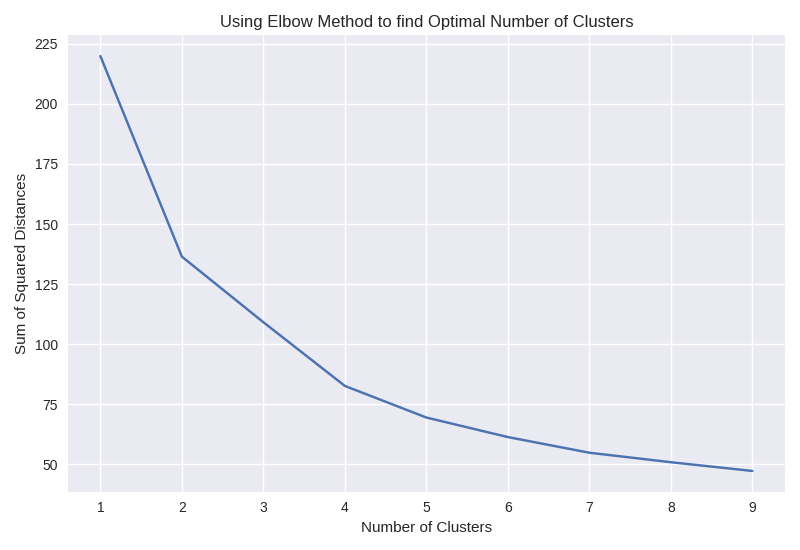
\includegraphics[width=\textwidth]{elbow}
\caption[Using Elbow Method to find Optimal Number of Clusters]{The Elbow Method runs the K-Means clustering algorithm with a range of clusters and computes the sum of squared errors. This sum measures how close the predicted clusters match the data points; the greater the error, the less clusters fit the data. This graph converges to 0 at $N$ clusters where each point is its own cluster and thus has zero error. To find an appropriate number of clusters, we need to visually find an \textquote{elbow} point on the graph, i.e. where adding an additional cluster will not significantly reduce the error. In this graph, the elbow point is at 4 clusters.}
\label{fig:ctm-num-clusters}
\end{figure}

%------------------------------------------------------------------------------
\subsubsection{Cleaning Up Data}
%------------------------------------------------------------------------------

Although not essential, we chose to perform Principal Component Analysis (PCA) \cite{wold1987principal} on our data prior to clustering. PCA transforms our set of $M$ features into a smaller set of linearly uncorrelated features or \textquote{components}. The components are sorted in descending order of variance. In other words, the first few components theoretically capture the majority of the \textquote{information} in the source data.

The most obvious advantage of PCA is reducing the runtime of our clustering algorithms because it eliminates features (columns in our data matrix) that represent very little information about our data points. This technique is also useful in visualization as it allows high-dimensional data to be presented in a 2D graph while preserving the majority of the information and relationships between data points.

To use PCA, we need to specify how many components or features to keep. Similar to the Elbow Method to determine the number of clusters, we can look at the graph of cumulative explained variance shown in Figure~\ref{fig:ctm-num-components} to estimate an appropriate number of components. For our data, the graph recommended for us to use 6 components.

\begin{figure}
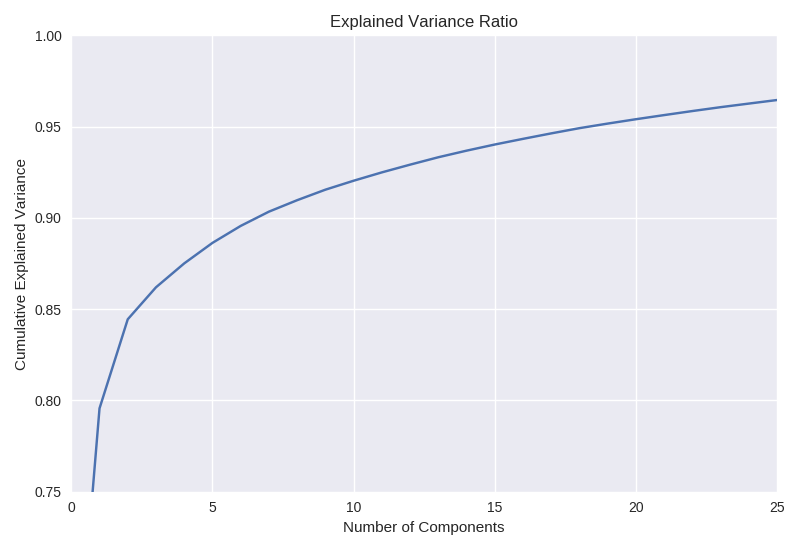
\includegraphics[width=\textwidth]{explained_variance_ratio}
\caption[Explained Variance Ratio]{The explained variance conceptually represents the amount of information in the original data that each component captures. The first component captures almost 80\% of the original information; the second component captures another 5\%; and so on. This graph show the cumulative explained variance that each additional component captures. A rule-of-thumb for PCA is to choose the number of components at an \textquote{elbow point} where adding an additional component will not capture significantly more information. In this graph, the elbow point is at 6 components.}
\label{fig:ctm-num-components}
\end{figure}

\subsection{K-Means}
\label{sec:ctm-km}

The first clustering algorithm we tried was K-Means \cite{macqueen1967some}. It iteratively tries to group unlabeled data points with similar features together by minimizing the mean distance between each point in each group. Figure~\ref{fig:ctm-km} visualizes the groups labeled by the K-Means algorithm on the 2017 class for the Non-Blocking IO assignment.

The K-Means algorithm constructs each group to minimize the average distance from the group's centroid to every point in its corresponding group. Since the majority of students in our data set received full marks, we assumed the majority of the data points in each group should also represent full-mark solutions. As a result, the volume of full-mark solution points should draw the centroid of each group towards \textquote{regions} representing higher marks. Based on this idea, we calculated a student's score based on their distance to their corresponding group's centroid; the closer a student was to their group's centroid, the higher their probability of receiving a high score.

Let $P_i$ denote the point representing student $i$ and $C_i$ denote the centroid of the student's group. The distance from centroid $d_i$ is defined as:
\begin{equation*}
d_i = \norm{P_i - C_i}
\end{equation*}

As mentioned in Figure~\ref{fig:ctm-km}, the scales in the axes have no tangible interpretations. Therefore, the distances from centroid $d_i$ we calculated for each point also had no meaningful interpretation. As a result, we tried to evaluate each point's centroid distance relative to all other points. In other words, we calculated each student's score based on their performance relative to the rest of their class.

Let $\mu$ denote the mean and $\sigma$ denote the standard deviation of centroid distances of every student. We calculated student $i$'s score as follows:
\begin{equation*}
\text{Score}_i = 100 - 20 \cdot \frac{\abs{d_i - \mu}}{\sigma}
\end{equation*}

This equation deducted up to 20 points for each standard deviation of centroid distance a student was from their corresponding group's centroid. We chose to deduct 20 points per standard deviation arbitrarily after experimenting with different values. The main idea was to deduct marks based on how far the solution was from the centroid, where we assumed majority of the full mark solutions were located.

\begin{figure}
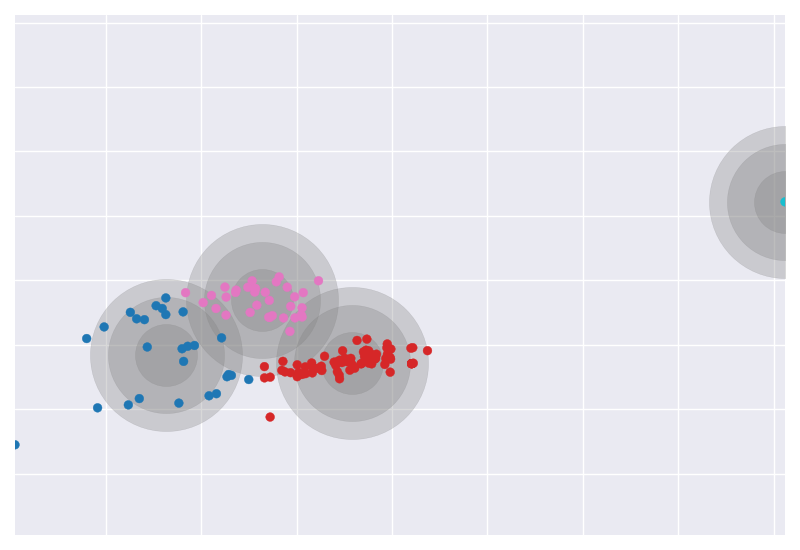
\includegraphics[width=\textwidth]{conversion-to-mark/marking_paster_nbio_ece459-a1-w2017_km}
\caption[K-Means Clustering]{Each data point represents a student solution to the Non-Blocking IO assignment from the 2017 class. It is important to note that this is a 2D projection of a multidimensional data set. Since we preprocessed the data with PCA, the first two dimensions presented here already capture the majority of the data variance. The scales in the axes are omitted because they have no tangible interpretations; they are meant for interpreting relative distances. The K-Means algorithm assigned each point a group, represented by their corresponding colour. Each set of concentric circles represent an arbitrary distance from the centroid of each group.}
\label{fig:ctm-km}
\end{figure}

\subsection{Gaussian Mixture}
\label{sec:ctm-gm}

The second clustering algorithm we tried was Gaussian Mixture \cite{dempster1977maximum}. Similar to the K-Means algorithm, it also groups unlabeled data points but with different criteria. As its name suggests, it assumes the points are randomly distributed following a Gaussian distribution. It iteratively tries to assign groups to maximize the likelihood of each data point belonging to their assigned groups. Likewise, we hypothesized that the closer a point (student solution) is to the centroid, in this case the central probability contour, the higher the probability of the student receiving a high score. In practice, we designated each student's score to be equal to the probability of them belonging to their assigned cluster, returned from the Gaussian Mixture algorithm.

\begin{figure}
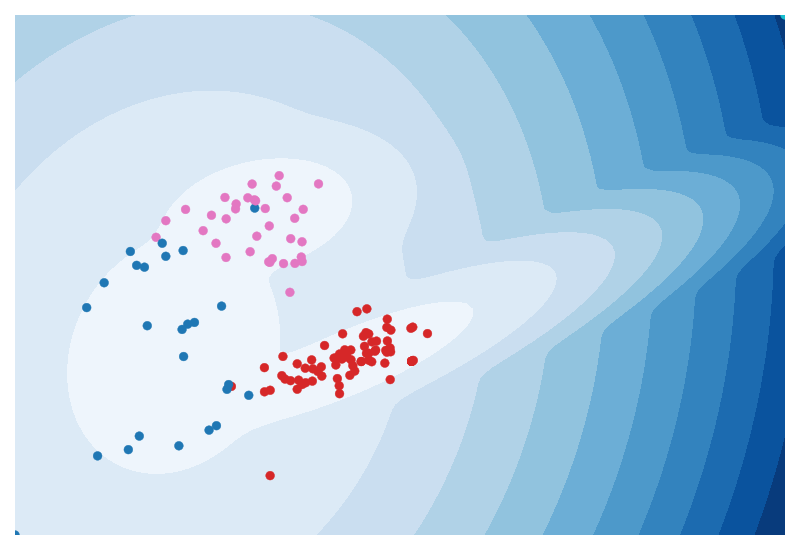
\includegraphics[width=\textwidth]{conversion-to-mark/marking_paster_nbio_ece459-a1-w2017_gm}
\caption[Gaussian Mixture Clustering]{This is a probability contour graph of our data points grouped by the Gaussian Mixture algorithm. Points closer to the center of the contours, i.e. lighter areas, have a higher probability of belonging to their corresponding group.}
\label{fig:ctm-gm}
\end{figure}

\subsection{HDBSCAN}
\label{sec:ctm-hdb}

The third and last clustering algorithm we experimented with was HDBSCAN (Hierarchical Density-Based Spatial Clustering of Applications with Noise) \cite{McInnes2017}. Similar to the previous two algorithms, it tries to group unlabeled data points with its own set of criteria. As its name implies, it tries to group points based on spatial density to ensure the resulting groups meet some density parameter.

The advantage of HDBSCAN is that it does not require us to specify the number of clusters we want to find. Instead, we specify the minimum number of points in each cluster $P$ and the algorithm will dynamically group points such that the resulting clusters have at least $P$ points. This gives us more flexibility in our parameters because choosing the number of clusters is harder than choosing the minimum number of points per cluster. We do not know the proper the number of clusters and thus must estimate it through an ad-hoc procedure. However, we do have a stronger conceptual understanding of the number of points per cluster: since we know there are only a limited number of approaches to solve an assignment and we know the majority of the students will follow similar approaches, either through collaboration or coincidence due to limited unique approaches, we know the $P$ value must be a significant fraction of the total number of students.

However, the disadvantage of this algorithm is that it is not guaranteed to be able to label every point; outlier points that cannot satisfy the group's density criteria are discarded as noise. The higher the minimum cluster size parameter $P$, the more points will be unlabeled. Ideally we want our groups to be as dense as possible so that we know the grouped points are extremely similar to each other. Ultimately, it is a balance between how many points we can label (automation rate) and how dense the resulting groups are.

Figure~\ref{fig:ctm-hdb} shows how the algorithm labels our data set based on varying minimum cluster sizes. A cluster size of 5 is able to achieve 3 groups, which is close to the 4 groups set for the previous two algorithms. However as we can see from the graph, the 3 groups are slightly sparse. As a result, we chose $P=10$ because it is able to label most of the points without sacrificing too much density; at higher cluster sizes, we do not seem to significantly increase our groups' densities.

Once we were satisfied with our parameters, we ran the HDBSCAN algorithm and designated each student's score to be equal to the \textquote{strength} of the student's corresponding group prediction returned from the algorithm.

\begin{figure}
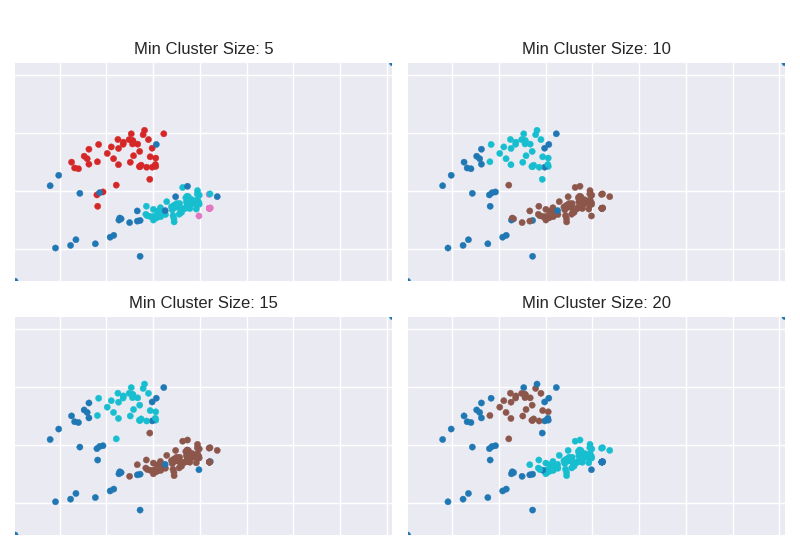
\includegraphics[width=\textwidth]{conversion-to-mark/marking_paster_nbio_ece459-a1-w2017_hdb}
\caption[HDBSCAN Clustering]{These graphs show our data points clustered with HDBSCAN using different minimum cluster size parameters. The higher the minimum size, the denser the resulting clusters. Furthermore, higher cluster sizes also result in more outlier points marked as noise (dark blue) as well as fewer total clusters. Cluster size of 5 has three different groups whereas cluster sizes of 10 and higher only have two different groups.}
\label{fig:ctm-hdb}
\end{figure}

